\documentclass[12pt]{article}

\usepackage{graphicx}

\setlength{\parskip}{1em}
\renewcommand{\baselinestretch}{2}

\title{Lab 03\\Multifunctional Logic Circuit\\ECE-380-002\\University of Alabama}
\author{Yichen Huang \\Thomas Dillman}
\date{2019/09/16}


\begin{document}
\maketitle
\newpage
\section{Introduction}

In Lab03, our team designed, built, and tested a multifunctional logic circuit that implements multiple logic functions.
We use the Quartus II CAD tool to design the circuit and write VHDL code. 
After compiled the files, we test the designs on Altera’s DE1 board and valid the outcome in the prelab truth table.

\section{Procedure}


\subsection{PreLab}

In the prelab, we firstly analyze the problem and finish the truth table of the function. 
We also make a K-Map of the function, calculate the function through minimum term method and build truth table. 
Finally, we draw the NAND-only schematic on the paper.
\begin{figure}[ht]
    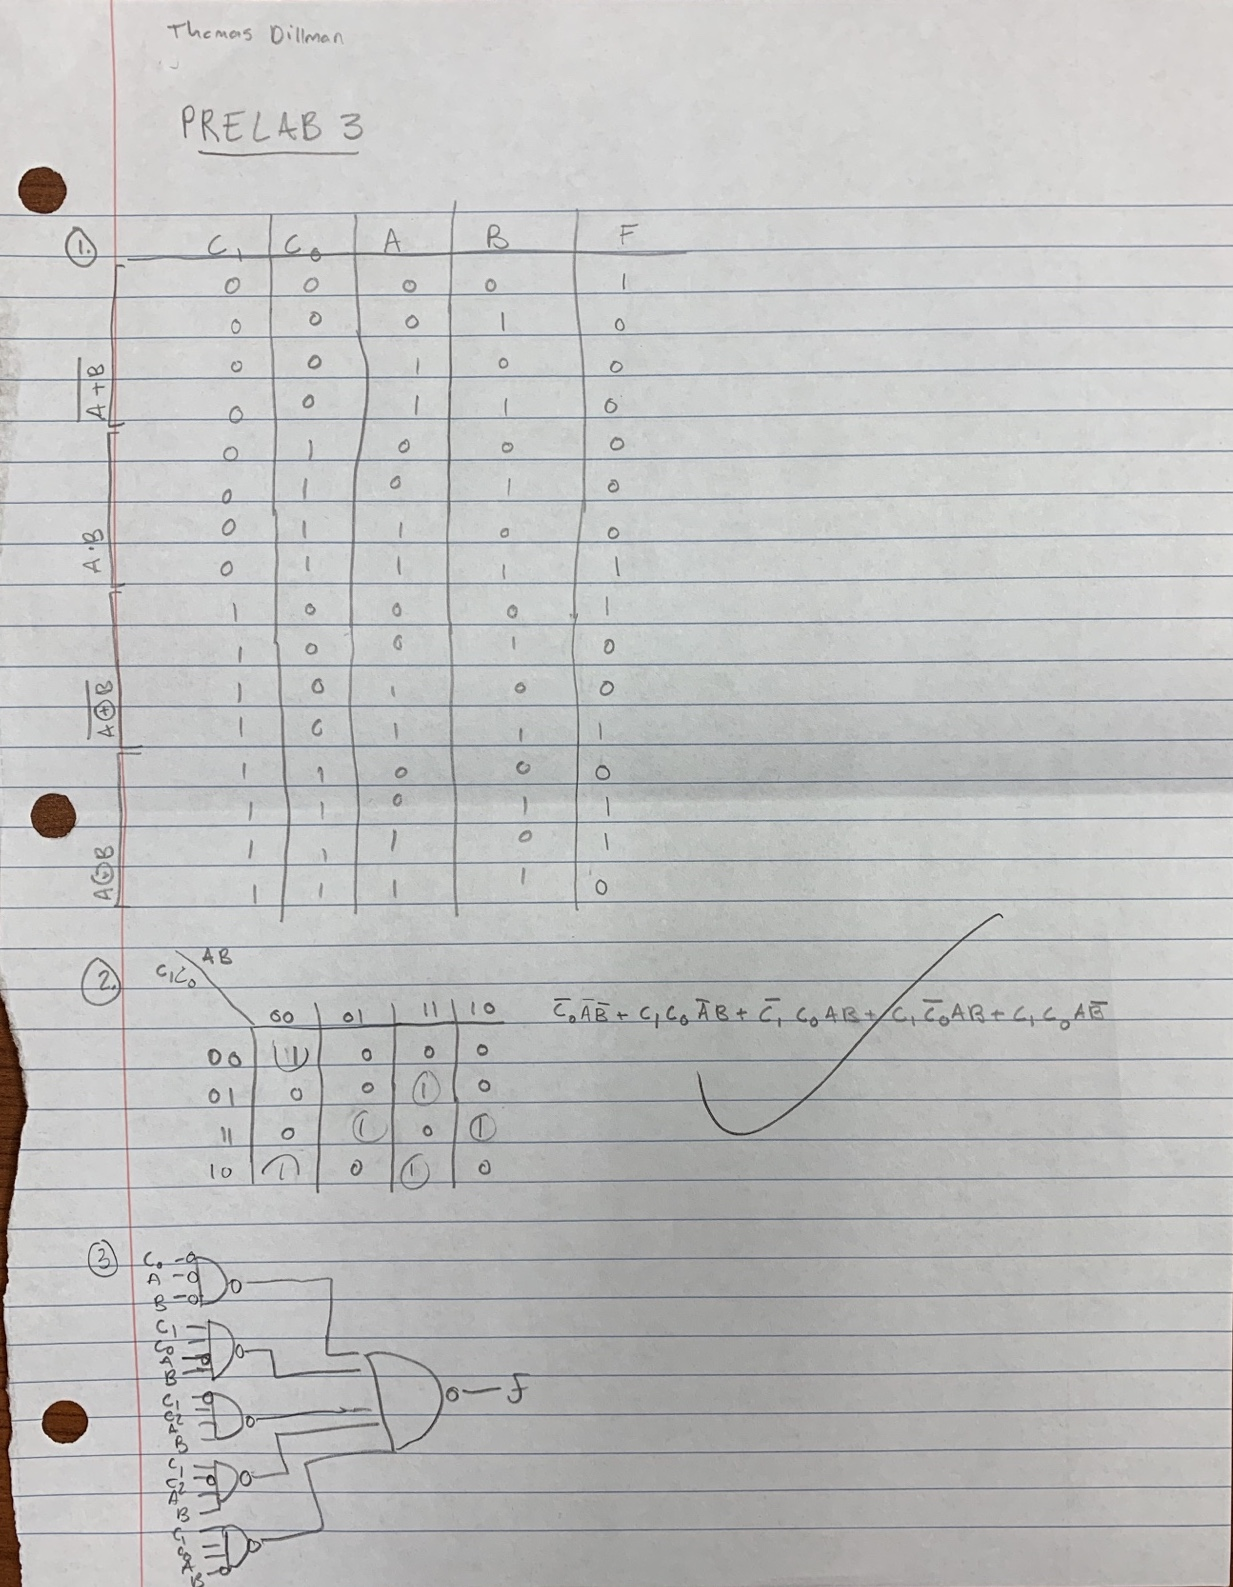
\includegraphics[scale=0.3]{Prelab3A.jpeg}
\end{figure}
\begin{figure}[ht]
    

    
\end{document}
